\documentclass[11pt]{article}

\usepackage[margin=1in]{geometry}
\usepackage[T1]{fontenc}
\usepackage[utf8]{inputenc}
\usepackage{lmodern}
\usepackage{microtype}
\usepackage{amsmath, amssymb}
\usepackage{booktabs}
\usepackage{array}
\usepackage{tabularx}
\usepackage{graphicx}
\usepackage{xcolor}
\usepackage{hyperref}
\usepackage{url}
\usepackage[numbers,sort&compress]{natbib}
\usepackage{titlesec}
\usepackage{pgfplots}
\pgfplotsset{compat=1.18}

\setlength{\parindent}{1.2em}
\setlength{\parskip}{0pt}
\setlength{\tabcolsep}{8pt}
\setlength{\textfloatsep}{10pt plus 2pt minus 2pt}
\setlength{\floatsep}{8pt plus 2pt minus 2pt}
\setlength{\intextsep}{8pt plus 2pt minus 2pt}
\raggedbottom
\newcolumntype{L}{>{\raggedright\arraybackslash}X}

\titleformat{\section}{\large\bfseries}{\thesection.}{0.6em}{}
\titleformat{\subsection}{\normalsize\bfseries}{\thesubsection.}{0.6em}{}
\titleformat{\paragraph}[runin]{\normalsize\bfseries}{}{0pt}{}[.]
\titlespacing*{\section}{0pt}{1.2em plus 0.2em minus 0.1em}{0.45em}
\titlespacing*{\subsection}{0pt}{0.9em plus 0.15em minus 0.1em}{0.3em}

\hypersetup{
  colorlinks=true,
  linkcolor=blue!50!black,
  citecolor=blue!50!black,
  urlcolor=blue!50!black
}

\begin{document}

\begin{center}
{\LARGE\bfseries Early Speech Emergence in a Small OLMo-Hybrid Speech Codec Language Model\par}
\vspace{0.35em}
{\large A 21.9M-Parameter LJ Speech Pilot\par}
\vspace{0.9em}
{\normalsize Micheal Ohagwu\par}
{\small \texttt{obioh@Icloud.com}\par}
\vspace{0.2em}
{\small March 2026\par}
\end{center}

\vspace{0.4em}

\begin{abstract}
We study whether a small OLMo-Hybrid-style recurrent-attention language model can learn speech codec structure well enough to produce clearly voice-like audio, without text conditioning, on a clean single-speaker corpus. The model operates over 8-codebook EnCodec 24~kHz tokens extracted from LJ Speech and uses an 8-layer decoder with a 3:1 recurrent-to-attention schedule, yielding 6 Gated DeltaNet blocks and 2 attention blocks for a total of 21.9M parameters. On an NVIDIA A100-SXM4-80GB, the best locally preserved checkpoint reached an EMA validation loss of 4.2847 and perplexity 72.58 at step 1800, before pod failure interrupted the run near the step-2000 boundary. Direct listening to fixed-prompt local samples from steps 1200, 1400, 1600, and 1800 showed a clear speaking timbre and speech-like local structure, with failures dominated by babble and weak articulation rather than static, drone noise, or codec collapse. The stable run did not use the intended fused Flash Linear Attention Gated DeltaNet kernel due upstream Triton/kernel failures, so the reported systems performance is conservative relative to the architecture's intended fast path. We present this result as a pilot study: not a benchmark claim, but evidence that an OLMo-Hybrid / Gated-DeltaNet-style backbone is a viable speech codec language model at small scale.
\end{abstract}

\section{Introduction}
Recent open work has revived interest in hybrid backbones that mix attention with modern recurrent or state-space layers, rather than treating transformers and recurrence as mutually exclusive design choices \citep{merrill2026olmohybrid, yang2024gateddeltanet}. In parallel, speech generation work has shown that neural audio codecs and token language models are a practical route to naturalistic speech and audio synthesis \citep{borsos2022audiolm, defossez2022encodec, wang2023valle, zhang2023speechtokenizer}. The obvious next question is whether these ideas combine well: can a small hybrid recurrent-attention backbone model speech codec tokens effectively enough to produce clearly voice-like samples?

This report documents a deliberately narrow pilot designed to answer that question. We did \emph{not} attempt to build a full text-to-speech system, a streaming agent, or a production voice model. Instead, we asked a threshold question:

\begin{quote}
Can a compact OLMo-Hybrid-style decoder trained unconditionally on speech codec tokens cross the boundary from static or decoder garbage into clearly voice-like output?
\end{quote}

That threshold matters because it separates architecture and pipeline viability from final product quality. If the model cannot produce anything beyond hiss, drone artifacts, or obvious tokenization failure, then text conditioning, speaker conditioning, or larger-scale training are premature. If it \emph{can} produce voice-like babble at small scale, then the architecture is at least plausible for more serious follow-up work.

Our main result is modest but real: on LJ Speech \citep{ito2017ljspeech}, a 21.9M-parameter OLMo-Hybrid-style speech codec LM trained on EnCodec 24~kHz tokens \citep{defossez2022encodec} produced clear voice-like audio by step 1800 on an A100, despite (i) no text conditioning, (ii) no fused recurrent FLA kernel, and (iii) termination well before the planned 12k-step budget. To our knowledge, public speech token language modeling work has focused primarily on transformer-heavy or pure state-space backbones \citep{borsos2022audiolm, wang2023valle, zhang2023speechtokenizer, lu2025duplexmamba}; we are not aware of a prior public pilot centered on an OLMo-Hybrid / Gated-DeltaNet-style backbone for speech codec language modeling.

We therefore position this document as a technical report, not a benchmark paper. Its contributions are:

\begin{enumerate}
    \item a concrete OLMo-Hybrid-style adaptation for speech codec LM, described at the level of block schedule, head geometry, token interface, and loss;
    \item a small but clean A100 pilot showing monotonic validation improvement through step 1800, reaching EMA validation loss 4.2847 and perplexity 72.58;
    \item qualitative evidence that the model learned voice-like local speech structure well before full convergence;
    \item an honest systems account of what did and did not work, including the stable no-FLA A100 path and the operational implications of pod volatility.
\end{enumerate}

\section{Related Work}
\paragraph{Hybrid recurrent-attention language models.}
OLMo Hybrid argues that hybrids mixing attention and linear RNN layers are not merely inference-efficient alternatives to transformers, but a more expressive family that can scale better in pretraining \citep{merrill2026olmohybrid}. Their released 7B model uses a 3:1 schedule of Gated DeltaNet and attention layers. The underlying recurrent operator, Gated DeltaNet, extends DeltaNet-style recurrence with gated parameterization, short causal convolutions, and a training-friendly formulation intended to pair with fused Flash Linear Attention kernels \citep{yang2024gateddeltanet}.

\paragraph{Speech token language modeling.}
AudioLM established that language models over discrete audio tokens can generate coherent speech and other audio without relying on text supervision \citep{borsos2022audiolm}. VALL-E framed zero-shot TTS as neural codec language modeling and showed that codec-token autoregression can produce high-quality conditional speech synthesis at scale \citep{wang2023valle}. SpeechTokenizer argued that tokenizers designed for speech language modeling can outperform generic alternatives and paired them with a Unified Speech Language Model \citep{zhang2023speechtokenizer}. On the state-space side, DuplexMamba explored Mamba-based speech interaction, but in a duplex streaming speech-to-text conversation setting rather than an unconditional speech codec LM \citep{lu2025duplexmamba}.

\paragraph{Token interleaving for multi-codebook generation.}
We train with a delay-pattern objective closely aligned with the multi-codebook interleaving popularized by MusicGen \citep{copet2023simple}: codebook $k$ is shifted by $k$ positions so that a single autoregressive step predicts one token per codebook on a staircase-shaped frontier.

\section{Model}
\subsection{Overview}
The model is a decoder-only language model over residual vector quantization (RVQ) codes. Audio is tokenized into $K=8$ EnCodec codebooks; the model consumes delay-patterned tokens and predicts the next delayed token autoregressively. Table~\ref{tab:arch} summarizes the configuration.

\begin{table}[t]
    \centering
    \caption{Architecture and training configuration for the stable A100 run.}
    \label{tab:arch}
    \begin{tabularx}{0.92\linewidth}{@{}lL@{}}
        \toprule
        Item & Value \\
        \midrule
        Total parameters & 21,904,648 \\
        Embedding parameters & 3,154,944 \\
        Backbone parameters & 15,594,376 \\
        Output-head parameters & 3,155,328 \\
        Layers & 8 \\
        Width & $d_{\text{model}}=384$ \\
        FFN width & $d_{\text{ff}}=1024$ \\
        Attention heads & 6 \\
        KV heads & 2 \\
        Attention schedule & every 4th block, final block forced to attention \\
        Block mix & 6 Gated DeltaNet + 2 attention \\
        Dropout & 0.1 \\
        Max sequence length & 1024 delayed steps \\
        Codebooks / vocab & 8 / 1027 \\
        Codec & EnCodec 24~kHz, 6.0 kbps \\
        Chunk length & 8.0 s \\
        Batch size & 24 \\
        Optimizer & fused AdamW, $\beta=(0.9,0.95)$, weight decay 0.01 \\
        Schedule & warmup 500, cosine decay from $3\times10^{-4}$ to $10^{-5}$ \\
        Precision & bfloat16 \\
        \bottomrule
    \end{tabularx}
\end{table}

\subsection{Token interface and delay pattern}
Let raw codec tokens be $z \in \{0,\dots,V-1\}^{K \times T}$ with $K=8$ codebooks and vocabulary $V=1027$ including special tokens. We apply a delay pattern $\Delta$:
\[
\tilde{z}_{k,t} =
\begin{cases}
z_{k,t-k} & \text{if } 0 \le t-k < T,\\
\texttt{PAD} & \text{otherwise,}
\end{cases}
\]
so the model predicts a staircase of codebook targets rather than all raw codebooks aligned at the same step. For our 8-second EnCodec chunks, local sample metadata confirmed an effective frame rate of approximately 75~Hz, so a 600-frame raw chunk becomes 607 delayed steps. The 1024-step context therefore covers the full 8-second training chunk without truncation.

\subsection{Backbone}
The backbone follows the public OLMo Hybrid pattern \citep{merrill2026olmohybrid}: three recurrent blocks followed by one attention block, repeated across the network, with the final layer forced to attention. In this 8-layer instance, the schedule is:
\[
[\text{GDN}, \text{GDN}, \text{GDN}, \text{Attn}, \text{GDN}, \text{GDN}, \text{GDN}, \text{Attn}].
\]

Each block is pre-norm with RMSNorm, mixer, residual add, RMSNorm, SwiGLU MLP, residual add. RVQ embeddings are summed across codebooks at each delayed step to form a single 384-dimensional token representation; there is no learned absolute positional embedding.

\subsection{Attention blocks}
Attention blocks use grouped-query attention with 6 query heads and 2 KV heads, so the attention head dimension is $384 / 6 = 64$. Queries and keys are normalized with per-head RMSNorm, rotary position embeddings use $\theta = 500{,}000$, and PyTorch scaled dot-product attention is used on the fast CUDA path.

\subsection{Gated DeltaNet blocks}
The recurrent blocks implement a paper-aligned Gated DeltaNet-style mixer. Relative to the attention geometry, the recurrent blocks shrink the $q/k$ head width and expand the value width:
\[
d_{qk}^{\text{GDN}} = 0.75 \times 64 = 48,\qquad d_{v}^{\text{GDN}} = 2 \times 48 = 96.
\]
For each timestep, the block forms $q$, $k$, $v$, and gating signals $a$, $b$, together with learnable $A_{\log}$ and $\texttt{dt\_bias}$ parameters and short depthwise causal convolutions over the projected sequences. In the plain recurrent scan actually used for stable training, the state update is:
\begin{align}
r_t &= S_{t-1} k_t, \\
S_t &= \alpha_t \odot \left(S_{t-1} - \beta_t \odot (r_t k_t^\top)\right) + \beta_t \odot (v_t k_t^\top), \\
y_t &= S_t q_t,
\end{align}
with L2-normalized $q_t$ and $k_t$, and with a gated RMSNorm output projection. This mirrors the intended Gated DeltaNet structure from the released OLMo-core implementation, but in the stable A100 run it executed through the plain PyTorch fallback rather than the fused FLA kernel.

\subsection{Objective}
The training objective is next-token cross-entropy on delayed tokens:
\[
\mathcal{L}(\theta) =
\frac{1}{N}
\sum_{k,t}
\mathrm{CE}\!\left(
p_{\theta}(\tilde{z}_{k,t+1}\mid \tilde{z}_{\le t}),
\tilde{z}_{k,t+1}
\right),
\]
ignoring pad positions and using label smoothing 0.1. This is an unconditional codec language model: there is no text prompt, no speaker embedding, and no semantic token stream.

\section{Data and Training Setup}
\subsection{Dataset}
We used LJ Speech \citep{ito2017ljspeech}, a clean single-speaker English corpus frequently used in TTS research. The appeal of LJ Speech for this pilot was not scale but cleanliness: if the goal is to determine whether the backbone can learn local speech structure, a narrow acoustic domain is preferable to a noisy heterogeneous corpus.

We tokenized the corpus into non-overlapping 8-second chunks and split at the utterance level to avoid train/validation leakage across chunks from the same source waveform. The resulting tokenized dataset contained 12,624 training files and 666 validation files.

\subsection{Codec and metadata}
The authoritative dataset metadata came from the generated \texttt{codec\_meta.json}: EnCodec 24~kHz, 8 codebooks, codebook size 1024, 6.0 kbps bandwidth, 8.0-second chunking. One copied run configuration retained stale fallback codec defaults unrelated to the actual run, so for this report we reconstructed the codec description from the dataset metadata and saved sample manifests rather than from the copied run config alone.

\subsection{Stable A100 run}
The stable run used:
\begin{itemize}
    \item one NVIDIA A100-SXM4-80GB GPU,
    \item bfloat16 mixed precision,
    \item true batch size 24,
    \item 8 dataloader workers with prefetch factor 4, pinned memory, and non-blocking transfers,
    \item fused AdamW,
    \item CUDA scaled dot-product attention flash path enabled,
    \item \texttt{torch.compile} disabled for the stable run,
    \item the fused recurrent FLA path disabled due backward-kernel instability on the available Triton stack.
\end{itemize}

An earlier batch-32 attempt ran out of memory. Smaller batch/accumulation combinations were also tried, but batch 24 with no accumulation was the best stable operating point found under the budget.

\subsection{A100 run chronology and operating-point search}
The final reported A100 result was not the first A100 launch. The practical training path involved a short search over operating points under tight budget constraints and unreliable pod infrastructure. The decisive run was:
\[
\texttt{ljspeech\_olmo\_hybrid\_a100\_no\_fla\_12k\_b24a1}.
\]

Before landing on that configuration, we explored more conservative and more aggressive operating points. Table~\ref{tab:a100-search} summarizes the relevant A100 configurations used during the search.

\begin{table}[t]
    \centering
    \caption{A100 operating-point search for the no-FLA training path.}
    \label{tab:a100-search}
    \begin{tabularx}{0.96\linewidth}{@{}l c l L@{}}
        \toprule
        Configuration & Effective batch & Outcome & Role in final result \\
        \midrule
        $8 \times 4$ & 32 & stable but underutilized & initial safe A100 launch \\
        $16 \times 2$ & 32 & stable, better utilization & intermediate tuning point \\
        $24 \times 1$ & 24 & stable, best practical tradeoff & \textbf{final reported run} \\
        $32 \times 1$ & 32 & out-of-memory / unstable & rejected \\
        \bottomrule
    \end{tabularx}
\end{table}

This operating-point search matters for interpretation. The reported A100 result is not merely ``an A100 run''; it is the outcome of choosing the largest stable no-FLA batch regime that fit the 80~GB card without sacrificing run survival. The run therefore reflects both architectural behavior and the systems reality of the unfused recurrent fallback.

\subsection{Systems caveat}
The intended fast path for the recurrent mixer was the fused Flash Linear Attention Gated DeltaNet kernel. In practice, the available pod/software stack failed in the fused backward kernel with Triton code-generation errors. As a result, the stable run reported here combines strong CUDA kernels for attention and optimization with an \emph{unfused recurrent fallback}. This matters for systems interpretation: the run demonstrates architectural viability, but not the architecture's best possible throughput on its intended kernel stack.

\section{Results}
\subsection{Validation trajectory}
Table~\ref{tab:eval-history} and Figure~\ref{fig:curves} summarize the recorded evaluation history up to the best locally preserved checkpoint.

\begin{table}[t]
    \centering
    \caption{Evaluation history from the stable A100 run.}
    \label{tab:eval-history}
    \begin{tabular}{@{}r r r r r r@{}}
        \toprule
        Step & Train loss & LR & Grad norm & EMA val loss & PPL \\
        \midrule
         200 & 5.0049 & $1.19{\times}10^{-4}$ & 0.28 & 6.7878 & 886.99 \\
         400 & 4.5167 & $2.39{\times}10^{-4}$ & 0.85 & 6.1530 & 470.13 \\
         600 & 4.2326 & $3.00{\times}10^{-4}$ & 0.18 & 5.6474 & 283.54 \\
         800 & 4.6158 & $3.00{\times}10^{-4}$ & 0.24 & 5.1973 & 180.78 \\
        1000 & 4.1367 & $2.99{\times}10^{-4}$ & 0.21 & 4.8510 & 127.87 \\
        1200 & 4.1702 & $2.97{\times}10^{-4}$ & 0.20 & 4.6169 & 101.18 \\
        1400 & 4.4976 & $2.96{\times}10^{-4}$ & 0.21 & 4.4626 & 86.72 \\
        1600 & 4.2774 & $2.94{\times}10^{-4}$ & 0.20 & 4.3585 & 78.14 \\
        1800 & 4.2224 & $2.91{\times}10^{-4}$ & 0.18 & \textbf{4.2847} & \textbf{72.58} \\
        \bottomrule
    \end{tabular}
\end{table}

\begin{figure}[t]
    \centering
    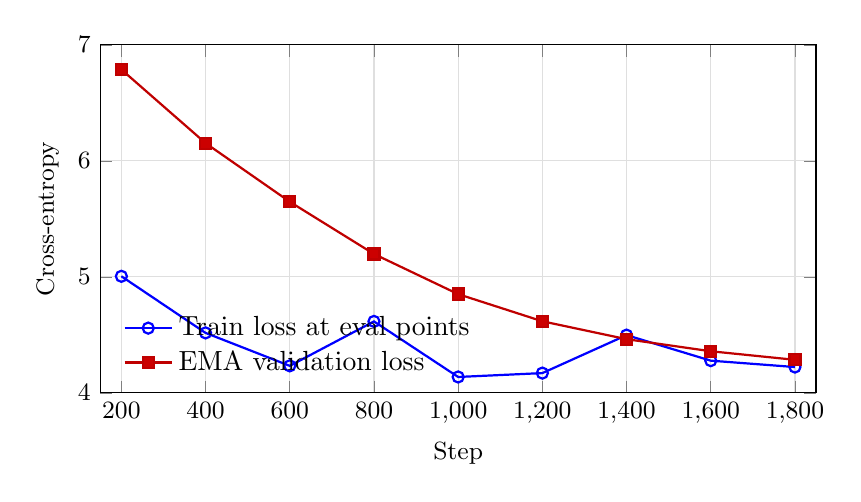
\begin{tikzpicture}
    \begin{axis}[
        width=0.88\linewidth,
        height=6.0cm,
        xlabel={Step},
        ylabel={Cross-entropy},
        xmin=150, xmax=1850,
        ymin=4.0, ymax=7.0,
        grid=both,
        minor grid style={gray!15},
        major grid style={gray!25},
        legend style={draw=none, fill=none, at={(0.02,0.02)}, anchor=south west},
        tick label style={font=\small},
        label style={font=\small},
        legend cell align=left
    ]
    \addplot+[blue, thick, mark=o] coordinates {
        (200,5.0049) (400,4.5167) (600,4.2326) (800,4.6158)
        (1000,4.1367) (1200,4.1702) (1400,4.4976) (1600,4.2774) (1800,4.2224)
    };
    \addlegendentry{Train loss at eval points}
    \addplot+[red!75!black, thick, mark=square*] coordinates {
        (200,6.7878) (400,6.1530) (600,5.6474) (800,5.1973)
        (1000,4.8510) (1200,4.6169) (1400,4.4626) (1600,4.3585) (1800,4.2847)
    };
    \addlegendentry{EMA validation loss}
    \end{axis}
    \end{tikzpicture}
    \caption{Training and validation loss over the stable A100 run. Validation improved monotonically through the best preserved checkpoint at step 1800.}
    \label{fig:curves}
\end{figure}

The best locally preserved checkpoint is the step-1800 model. The run likely reached or began the step-2000 boundary before the pod was torn down, but we did not recover a verified step-2000 checkpoint, so step 1800 is the final trusted result.

\subsection{Checkpoint chronology on the A100 run}
The saved checkpoint cadence was every 200 steps. The locally preserved A100 checkpoints therefore form a clean chronology of the actual run:
\[
200 \rightarrow 400 \rightarrow 600 \rightarrow 800 \rightarrow 1000 \rightarrow 1200 \rightarrow 1400 \rightarrow 1600 \rightarrow 1800.
\]
This chronology is not incidental. It is the concrete record of the best surviving A100 run, and it is the basis for the qualitative comparison bundles used later in the report. In particular, local artifacts were explicitly pulled for checkpoints 1200, 1400, 1600, and 1800 before the pod died. The best checkpoint through the surviving run history was the step-1800 model.

\subsection{Qualitative sampling protocol}
Qualitative evaluation was performed by direct listening to locally decoded 6-second continuations from checkpoints 1200, 1400, 1600, and 1800 under a fixed prompt and consistent sampling settings. Final qualitative probes used a corrected delay-space sampler rather than the earlier raw-code rollout that exaggerated timing artifacts. The improved local sampling settings were:
\begin{itemize}
    \item one raw seed frame from a held training chunk as prompt,
    \item duration 6.0 seconds,
    \item top-$p=0.9$,
    \item codebook-aware temperature schedule 0.72 $\rightarrow$ 0.55,
    \item codebook-aware top-$k$ schedule 48 $\rightarrow$ 24,
    \item repetition penalty 1.08 over a 48-token window.
\end{itemize}

\subsection{Qualitative outcome}
The key threshold was crossed well before full convergence. The outputs were \emph{not} static, hiss, or degenerate decoder noise. Instead, they exhibited:
\begin{itemize}
    \item a clearly human speaking timbre,
    \item local phonetic and prosodic structure,
    \item partial articulation and cadence,
    \item failure modes dominated by babble, weak semantics, and variable pacing.
\end{itemize}

This matters because it is a stronger result than merely reconstructing audio through the codec: the language model itself learned enough token dynamics to stay in the basin of ``speech-like'' output.

\subsection{Systems performance}
Throughput on the final A100 operating point was approximately 17.9k token-equivalents per second. This was substantially faster than the local M4 experiments, but still left the GPU underutilized relative to what the architecture should achieve with a working fused recurrent kernel. The reason is important: the bottleneck was not attention, dataloading, or basic CUDA support. It was the unfused recurrent Gated DeltaNet path. In other words, the run was good enough to validate the architecture, but not a definitive statement about the architecture's \emph{best} training efficiency.

This distinction was visible during the A100 search itself. Increasing the true batch improved memory occupancy and helped overall throughput, but did not produce the kind of saturation one would expect from a small dense transformer on the same hardware. That is exactly what one would expect when the dominant work is a recurrence-heavy plain PyTorch fallback instead of a fused recurrent kernel.

\section{Discussion}
The clearest positive conclusion is that the architecture worked. This may sound trivial, but for a pilot of a nonstandard backbone on speech codec tokens, it is not. By step 1800, the model had:
\begin{enumerate}
    \item learned a stable speech-like token distribution,
    \item improved validation monotonically up to the best preserved checkpoint,
    \item produced voice-like outputs under fixed local sampling,
    \item done so without text conditioning, speaker embeddings, or a semantic token hierarchy.
\end{enumerate}

That result is already enough to justify follow-up work. It suggests that the hybrid backbone is not merely ``compatible'' with speech codec LM in principle; it is \emph{practically viable} at small scale.

At the same time, the experiment does \emph{not} prove that this backbone is better than a matched transformer. We do not yet have the baseline needed to make that claim. What we can say is narrower:
\begin{itemize}
    \item the backbone is viable,
    \item the learning dynamics on the A100 run were clean,
    \item useful audio emerged early,
    \item the result is strong enough to motivate ablations, longer runs, and conditional extensions.
\end{itemize}

\section{Limitations and Threats to Validity}
This report has several important limitations.

\paragraph{No matched baseline.}
We did not run a same-parameter transformer baseline under the same data, tokenizer, and training budget. This prevents any claim of architectural superiority.

\paragraph{No human study.}
Qualitative evaluation was direct listening by the experimenter, not a blinded human evaluation with MOS, CMOS, or transcription-based intelligibility metrics.

\paragraph{Single-speaker data.}
LJ Speech is intentionally narrow. That is useful for isolating whether the architecture can learn speech structure, but it limits claims about general multi-speaker speech modeling.

\paragraph{No text conditioning.}
This was an unconditional codec LM. The report does not address pronunciation control, text alignment, or TTS quality.

\paragraph{Kernel mismatch.}
The stable run did not use the intended fused FLA recurrent path. The result therefore validates the model family more than it validates the final optimized training stack.

\paragraph{Pod volatility.}
The training environment was operationally fragile. Pod restarts changed SSH endpoints, local pod storage was not trustworthy, and the run likely died near the step-2000 boundary. We mitigated this by pulling checkpoints off-pod incrementally, but the final result is still shaped by infrastructure failure.

\section{Conclusion}
We presented a small-scale technical report on an OLMo-Hybrid-style speech codec language model trained unconditionally on LJ Speech tokenized with EnCodec 24~kHz. A 21.9M-parameter model with 6 Gated DeltaNet blocks and 2 attention blocks reached EMA validation loss 4.2847 and perplexity 72.58 by step 1800 on an A100, and direct listening confirmed clear voice-like outputs rather than static or decoder collapse. The model remained far from semantic or production-quality speech synthesis, but it definitively crossed the threshold that matters for a pilot: the backbone learned enough local speech structure to make the project worth continuing.

The next steps are straightforward:
\begin{enumerate}
    \item a matched transformer baseline,
    \item a longer run beyond 1800 steps,
    \item text conditioning,
    \item a more formal qualitative and quantitative evaluation,
    \item and eventually a fully fused recurrent kernel stack.
\end{enumerate}
If those follow-ups hold, this pilot will have served its purpose: not as a finished speech system, but as the first clean proof that the architecture belongs in the speech-token modeling conversation.

\paragraph{Artifact note.}
The locally preserved artifacts include checkpoints at steps 1200, 1400, 1600, and 1800, the best checkpoint through 1800, and fixed-protocol sample bundles for later comparison. These artifacts were used directly in preparing this report.

\bibliographystyle{plainnat}
\bibliography{references}

\end{document}
